\apendice{Documentación de usuario}

\section{Introducción}

En este apartado se va a explicar como se usa la aplicación para los usuarios posibles. Estos se dividen en dos roles, los administradores y los usuarios.

\section{Requisitos de usuarios}

Todos los tipos de usuario requerirán tener un navegador compatible con \texttt{HTML 5} y conexión a Internet.

\section{Instalación}

Al tratarse de una aplicación web no se requiere una instalación. La instalación del servicio web se explica en el \hyperref[sec:instalacion]{Instalación en entorno GNU/Linux}.

\section{Manual del usuario}

En esta sección se explicarán como usar las distintas funcionalidades de la aplicación web.

\subsection{Identificación del usuario}

El primer paso para utilizar \textit{SmartBeds}, en adelante "la web", es \textbf{iniciar la sesión} para acceder a las funcionalidades de la misma. 

Todos los pasos del proceso se pueden ver en las figuras~\ref{fig:man_start}~y~\ref{fig:man_inicio} :
\begin{enumerate}
	\item Hacer clic en \textit{inicie sesión}.
	\item Introducir su nombre de usuario en el campo \textit{Nombre de usuario} y la contraseña en el campo \textit{Contraseña}.
	\item Hacer clic en \textit{Entrar}).
\end{enumerate} 

En el caso de que no posea un usuario, o no disponga de su contraseña, contacte con su administrador.

Tras iniciar sesión, si es un usuario del tipo administrador, ve a la sección \hyperref[sec:admin_tuto]{Usuario administrador}; en el caso de ser un usuario normal ve a la sección de \hyperref[sec:normal_tuto]{Usuario normal}.

\begin{figure}
	\centering
	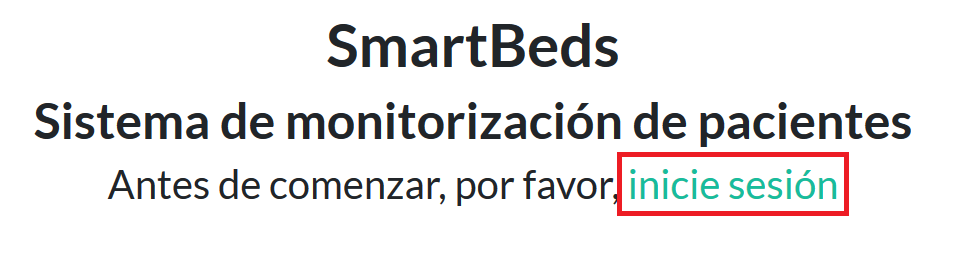
\includegraphics[width=0.8\textwidth]{manual/man_start}
	\caption{Manual: Ventana inicial.}
	\label{fig:man_start}
\end{figure}
\begin{figure}
	\centering
	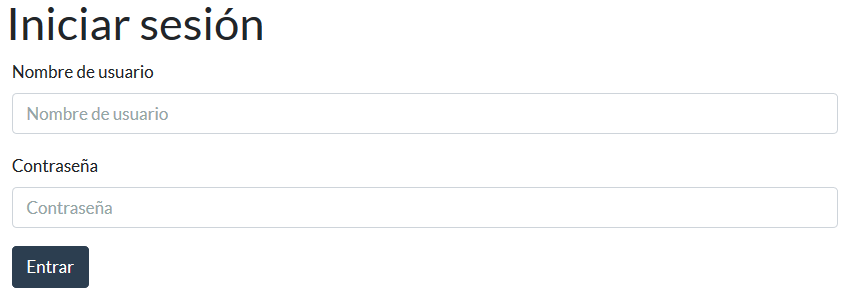
\includegraphics[width=0.8\textwidth]{manual/man_iniuser}
	\caption{Manual: Ventana de \textit{login}.}
	\label{fig:man_inicio}
\end{figure}

\subsection{Usuario administrador}\label{sec:admin_tuto}

En este apartado se encuentran las instrucciones para todas las funciones especiales del administrador. Las tareas comunes con el usuario normal se especifican en la sección~\ref{sec:normal_tuto}.

La \textbf{barra de navegación} es diferente para los administradores (Fig.~\ref{fig:man_nav}) incorporando los hiperenlaces a las tareas de administración.

\begin{figure}
	\centering
	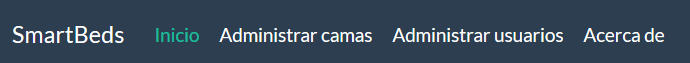
\includegraphics[width=\textwidth]{manual/man_navegacion}
	\caption{Manual: Barra de navegación de administrador.}
	\label{fig:man_nav}
\end{figure}

\subsubsection{Administración de camas}

Las tareas que se pueden realizar en la administración de camas son la \textbf{creación}, \textbf{modificación} y \textbf{eliminación} de camas así como la \textbf{gestión de permisos} relacionando la visibilidad de cada cama con cada usuario.  Para poder realizar esta administración se debe hacer clic al enlace \textit{Administrar camas} de la barra de navegación (Fig.~\ref{fig:man_nav}). La ventana de gestión de las camas se puede ver en la figura~\ref{fig:man_menu_cama}.

\begin{figure}
	\centering
	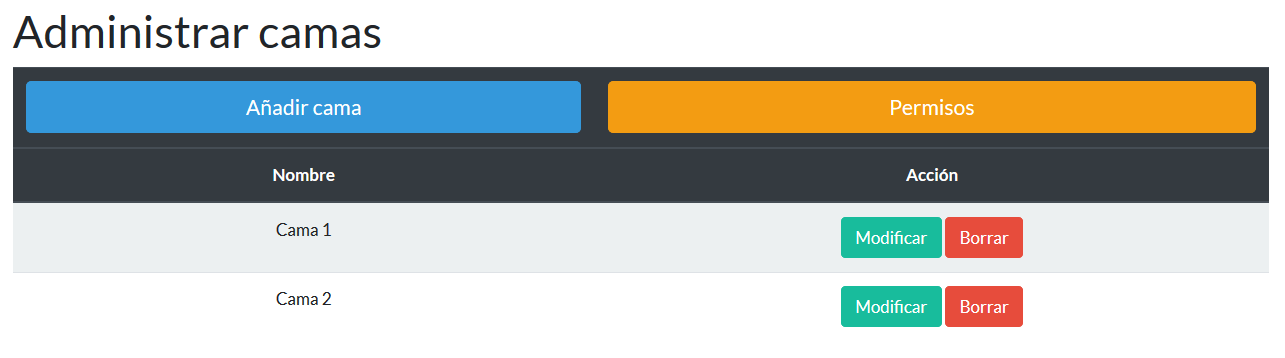
\includegraphics[width=\textwidth]{manual/man_gesbed}
	\caption{Manual: Administración de las camas.}
	\label{fig:man_menu_cama}
\end{figure}

Los pasos para la \textbf{creación de una cama} son los siguientes:
\begin{enumerate}
	\item Hacer clic en \textit{Añadir cama}.
	\item Rellenar los campos del formulario como se puede ver en la figura~\ref{fig:man_new_bed}. Hay que tener en cuenta que:
	\begin{itemize}
		\item Todos los campos son obligatorios.
		\item La ip ha de ser \texttt{MULTICAST}, es decir estar entre \texttt{224.0.0.0} y \texttt{239.255.255.255}.
		\item La dirección \texttt{MAC} y \texttt{UUID} han de ser ambos un valor hexadecimal sin ningún símbolo adicional (guiones, dos puntos etc.).
	\end{itemize}
	\item Solamente cuando esté bien cumplimentado se podrá hacer clic en \textit{Guardar cambios}.
\end{enumerate}

\begin{figure}
	\centering
	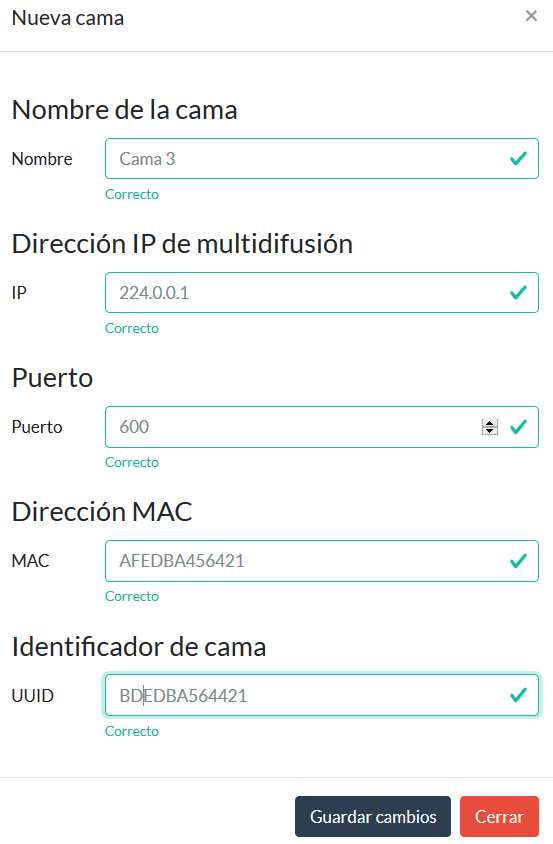
\includegraphics[width=0.7\textwidth]{manual/man_nueva}
	\caption{Manual: Crear cama.}
	\label{fig:man_new_bed}
\end{figure}

Los pasos para \textbf{modificar} los datos de una cama son:
\begin{enumerate}
	\item Hacer clic en el botón \textit{Modificar} de la cama deseada.
	\item Modificar los datos según se necesite, un ejemplo es la figura~\ref{fig:man_mod_bed}. La validación del formulario es igual que en la creación.
	\item Hacer clic en \textit{Guardar cambios}.
\end{enumerate}

\begin{figure}
	\centering
	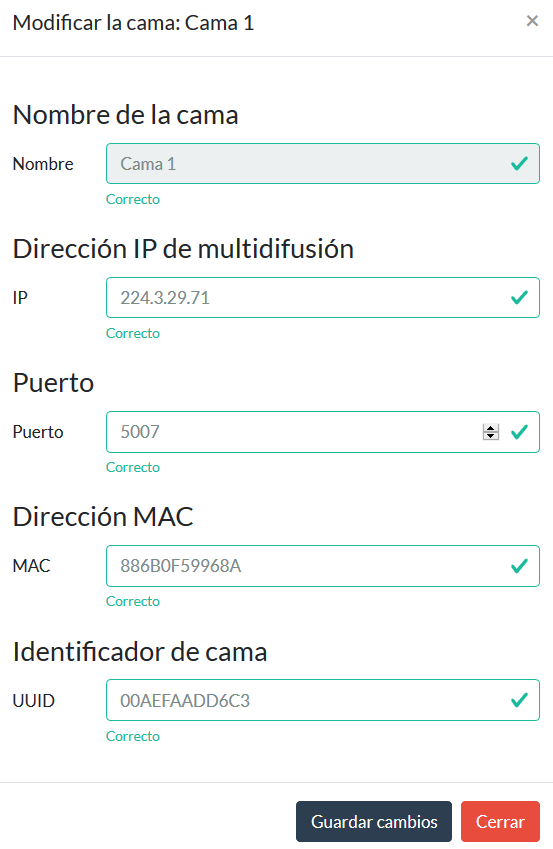
\includegraphics[width=0.7\textwidth]{manual/man_modificar}
	\caption{Manual: Modificar cama.}
	\label{fig:man_mod_bed}
\end{figure}

Para \textbf{borrar} una cama se necesitan los siguientes pasos:
\begin{enumerate}
	\item Hacer clic en \textit{Borrar} de la cama que se desee.
\end{enumerate}

Estas tres funcionalidades, debido a que no se disponen de camas físicas reales que se puedan escuchar, se han limitado para esta versión, por tanto, cualquiera que sea el proceso realizado no se completará ya que se recibirá el error de la figura~\ref{fig:man_error_no_dis}.

\begin{figure}
	\centering
	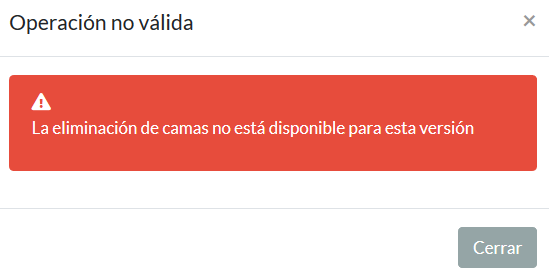
\includegraphics[width=0.7\textwidth]{manual/man_op_not}
	\caption{Manual: Error al crear, modificar o borrar una cama.}
	\label{fig:man_error_no_dis}
\end{figure}

La \textbf{modificación de los permisos} se realiza con los siguientes pasos:
\begin{enumerate}
	\item Hacer clic en \textit{Permisos}.
	\item Hacer clic en las cajas según se quiera dar o quitar permisos (Fig.~\ref{fig:man_perm}).
\end{enumerate}

\begin{figure}
	\centering
	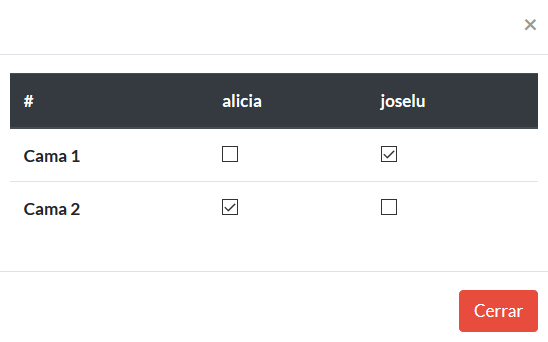
\includegraphics[width=0.7\textwidth]{manual/man_permisos}
	\caption{Manual: Tabla de permisos por usuario.}
	\label{fig:man_perm}
\end{figure}

\subsubsection{Administración de usuarios}

Las tareas que se pueden realizar en la administración de usuarios son la \textbf{creación}, \textbf{modificación de contraseña} y \textbf{eliminación} de usuarios. Para poder realizar esta administración se debe hacer clic al enlace \textit{Administrar usuarios} de la barra de navegación (Fig.~\ref{fig:man_nav}). La ventana de gestión de las camas se puede ver en la figura~\ref{fig:man_menu_usuario}

\begin{figure}
	\centering
	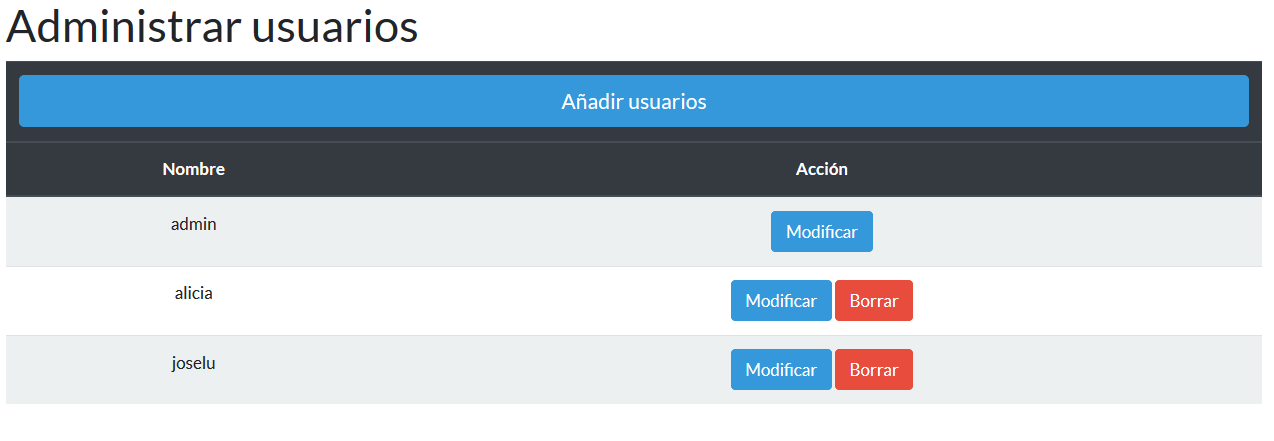
\includegraphics[width=\textwidth]{manual/man_user_menu}
	\caption{Manual: Administración de los usuarios.}
	\label{fig:man_menu_usuario}
\end{figure}

Los pasos para la \textbf{creación de un usuario} son:
\begin{enumerate}
	\item Hacer clic en \textit{Añadir usuarios}.
	\item Rellenar el formulario (Fig.~\ref{fig:man_new_user}), el \textit{nickname} ha de tener de tamaño máximo 50 caracteres.
	\item Hacer clic en \textit{Guardar cambios}.
\end{enumerate}

\begin{figure}
	\centering
	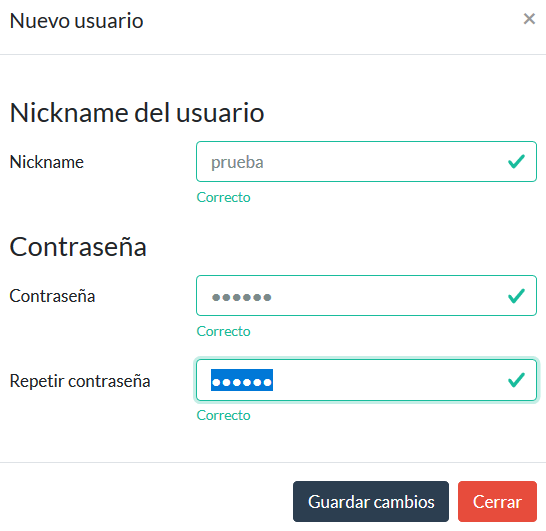
\includegraphics[width=0.7\textwidth]{manual/man_user_new}
	\caption{Manual: Formulario de creación de usuario.}
	\label{fig:man_new_user}
\end{figure}

Los pasos para \textbf{modificar la contraseña de un usuario} son:
\begin{enumerate}
	\item Hacer clic en \textit{Modificar} del usuario deseado.
	\item Rellenar el formulario (Fig.~\ref{fig:man_mod_user}).
	\item Hacer clic en \textit{Guardar cambios}
\end{enumerate}

\begin{figure}
	\centering
	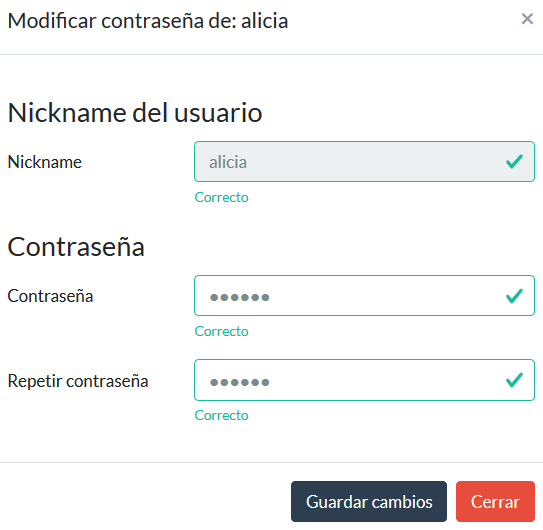
\includegraphics[width=0.7\textwidth]{manual/man_user_mod}
	\caption{Manual: Formulario de modificación de usuario.}
	\label{fig:man_mod_user}
\end{figure}

Los pasos para \textbf{borrar un usuario} son:
\begin{enumerate}
	\item Hacer clic en \textit{Borrar} del usuario deseado.
\end{enumerate}

\subsection{Usuario normal}\label{sec:normal_tuto}

La primera página que un usuario que se ha identificado es la lista de camas disponibles y su estado (Fig.~\ref{fig:man_bedlist}). Haciendo clic en cualquiera de los botones accederá a la página de esa cama (Fig.~\ref{fig:man_bed}). En la parte izquierda puede ver las constantes vitales, estos son:
\begin{itemize}
	\item \textbf{HR}: \textit{Hearth rate}, frecuencia cardíaca en pulsaciones por minuto.
	\item \textbf{RR}: \textit{Respiration rate}, frecuencia respiratorias en respiraciones por minuto.
	\item \textbf{SV}: \textit{Stroke volume}, volumen sistólico en mililitros.
	\item \textbf{HRV}: \textit{Heart rate variability}, variabilidad de la frecuencia cardíaca en milisegundos.
	\item \textbf{B2B}: \textit{Betweenn two beats}, tiempo entre dos pulsaciones en milisegundos.
\end{itemize}

En la parte derecha se encuentran los valores de las presiones de los seis tubos de la cama. Las posiciones de estos tubos son:
\begin{itemize}
	\item \textbf{P1}: Cabeza.
	\item \textbf{P2}: Hombros.
	\item \textbf{P3}: Abdomen.
	\item \textbf{P4}: Cadera.
	\item \textbf{P5}: Rodillas.
	\item \textbf{P6}: Pies.
\end{itemize}

\begin{figure}
	\centering
	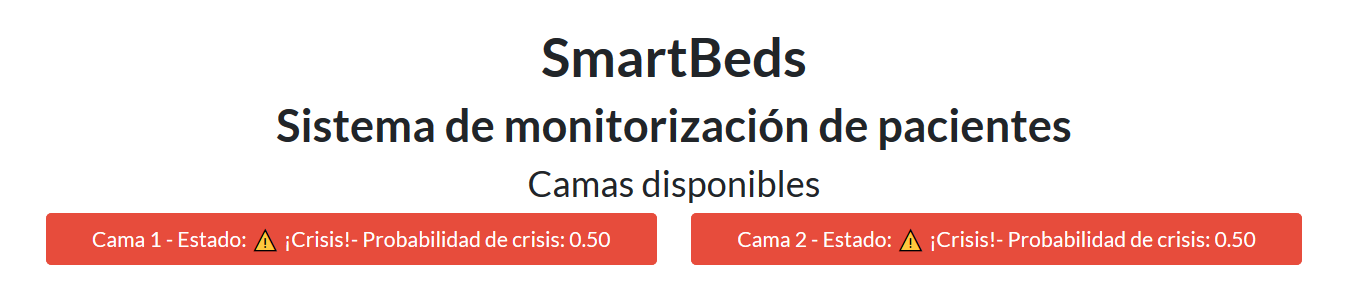
\includegraphics[width=\textwidth]{manual/man_allbeds}
	\caption{Manual: Formulario de modificación de usuario.}
	\label{fig:man_bedlist}
\end{figure}

\begin{figure}
	\centering
	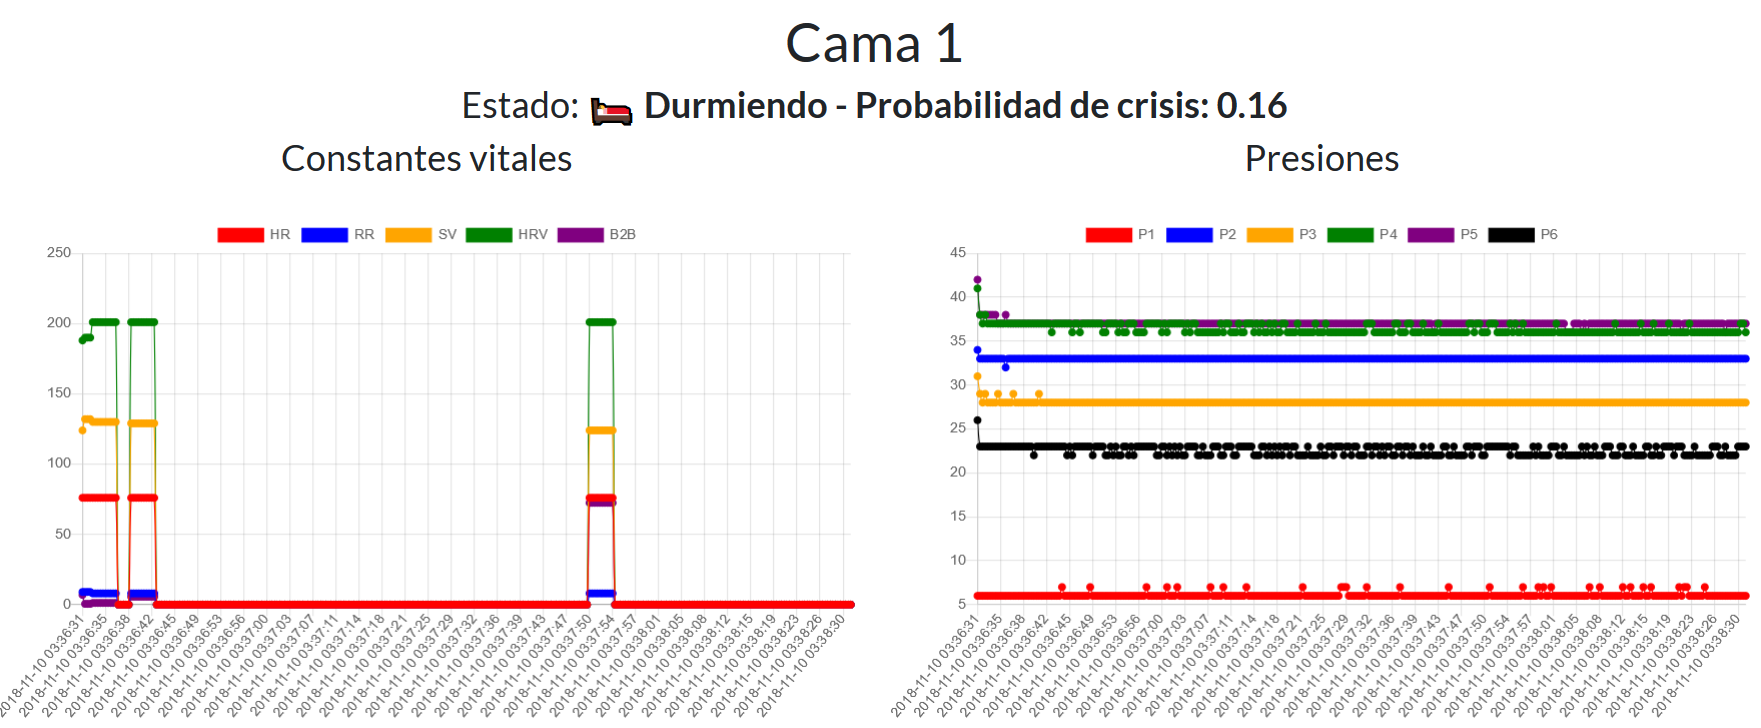
\includegraphics[width=\textwidth]{manual/man_cama1}
	\caption{Manual: Página con la información en tiempo real de una cama.}
	\label{fig:man_bed}
\end{figure}

La parte más importante es el \textbf{estado} del paciente, este puede ser dormido (Fig.~\ref{fig:man_dormido}), en una crisis (Fig.~\ref{fig:man_crisis}) o despierto (Fig.~\ref{fig:man_despiertos}). En las dos primeras situaciones incluye la probabilidad de una situación de crisis.

\begin{figure}
	\centering
	\begin{subfigure}[b]{0.48\textwidth}
		\centering
		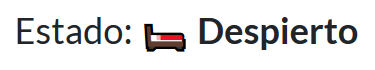
\includegraphics[width=1\textwidth]{manual/man_awake}
		\caption{Paciente despierto}
		\label{fig:man_despiertos}
	\end{subfigure}
	\begin{subfigure}[b]{1\textwidth}
		\centering
		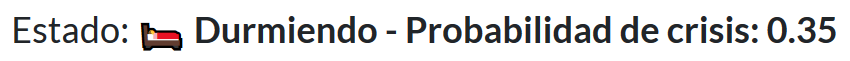
\includegraphics[width=1\textwidth]{manual/man_sleep}
		\caption{Paciente durmiendo}
		\label{fig:man_dormido}
	\end{subfigure}
	\begin{subfigure}[b]{0.9\textwidth}
		\centering
		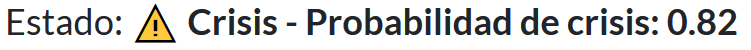
\includegraphics[width=1\textwidth]{manual/man_seizure}
		\caption{Paciente en una crisis epiléptica}
		\label{fig:man_crisis}
	\end{subfigure}
	\caption{Manual: diferentes estados de un paciente}
	\label{fig:man_states}
\end{figure}

\subsubsection{Cambiar la contraseña}
Para cambiar la contraseña de su usuario se necesita hacer clic al nombre del usuario en la parte derecha (Fig.~\ref{fig:man_username}) y rellenar el formulario al que se  redirige (Fig.~\ref{fig:man_changepass}).

\begin{figure}
	\centering
	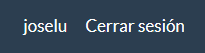
\includegraphics[width=0.4\textwidth]{manual/man_change1}
	\caption{Manual: Barra de navegación, lado derecho.}
	\label{fig:man_username}
\end{figure}

\begin{figure}
	\centering
	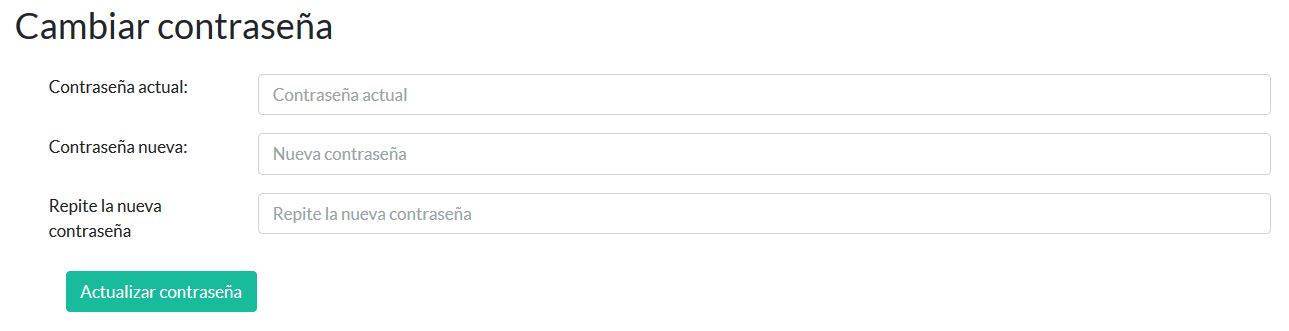
\includegraphics[width=\textwidth]{manual/man_change2}
	\caption{Manual: Formulario de cambio de contraseña.}
	\label{fig:man_changepass}
\end{figure}
